% This file was created with tikzplotlib v0.10.1.
\begin{tikzpicture}

\definecolor{darkorange25512714}{RGB}{255,127,14}
\definecolor{darkslategray38}{RGB}{38,38,38}
\definecolor{forestgreen4416044}{RGB}{44,160,44}
\definecolor{lightgray204}{RGB}{204,204,204}
\definecolor{steelblue31119180}{RGB}{31,119,180}

\begin{axis}[
axis line style={lightgray204},
height=0.45\textheight,
legend cell align={left},
legend style={fill opacity=0.8, draw opacity=1, text opacity=1, draw=none},
tick align=outside,
tick pos=left,
title={Relative execution times to C++},
width=\textwidth,
x grid style={lightgray204},
xlabel=\textcolor{darkslategray38}{Problem size},
xmajorgrids,
xmin=-5.35, xmax=134.35,
xtick style={color=darkslategray38},
y grid style={lightgray204},
ylabel=\textcolor{darkslategray38}{Execution time relative to C++},
ymajorgrids,
ymin=0.6, ymax=2.2,
ytick style={color=darkslategray38}
]
\path [draw=black, semithick]
(axis cs:1,1.21306956345733)
--(axis cs:1,1.28637933655133);

\path [draw=black, semithick]
(axis cs:2,1.13063718355118)
--(axis cs:2,1.15454712913278);

\path [draw=black, semithick]
(axis cs:4,0.857582528428346)
--(axis cs:4,0.989812920741126);

\path [draw=black, semithick]
(axis cs:8,0.968240592274161)
--(axis cs:8,1.01142042118736);

\path [draw=black, semithick]
(axis cs:16,0.963247757033249)
--(axis cs:16,0.991723214945013);

\path [draw=black, semithick]
(axis cs:32,0.974911442893033)
--(axis cs:32,0.998461759317531);

\path [draw=black, semithick]
(axis cs:64,0.95432553212862)
--(axis cs:64,1.01975373249419);

\path [draw=black, semithick]
(axis cs:128,0.963482123549343)
--(axis cs:128,1.01061798611725);

\path [draw=black, semithick]
(axis cs:1,1)
--(axis cs:1,1);

\path [draw=black, semithick]
(axis cs:2,1)
--(axis cs:2,1);

\path [draw=black, semithick]
(axis cs:4,1)
--(axis cs:4,1);

\path [draw=black, semithick]
(axis cs:8,1)
--(axis cs:8,1);

\path [draw=black, semithick]
(axis cs:16,1)
--(axis cs:16,1);

\path [draw=black, semithick]
(axis cs:32,1)
--(axis cs:32,1);

\path [draw=black, semithick]
(axis cs:64,1)
--(axis cs:64,1);

\path [draw=black, semithick]
(axis cs:128,1)
--(axis cs:128,1);

\path [draw=black, semithick]
(axis cs:1,0.828389558156663)
--(axis cs:1,0.876221553248934);

\path [draw=black, semithick]
(axis cs:2,1.16659640860399)
--(axis cs:2,1.18369956132969);

\path [draw=black, semithick]
(axis cs:4,0.812582689590874)
--(axis cs:4,0.942473738461775);

\path [draw=black, semithick]
(axis cs:8,0.94811121590957)
--(axis cs:8,0.986561064767915);

\path [draw=black, semithick]
(axis cs:16,0.932688005064488)
--(axis cs:16,0.961335728473359);

\path [draw=black, semithick]
(axis cs:32,0.88740876207216)
--(axis cs:32,0.913385818480991);

\path [draw=black, semithick]
(axis cs:64,1.04620045840618)
--(axis cs:64,1.12245437961835);

\path [draw=black, semithick]
(axis cs:128,1.04397360983739)
--(axis cs:128,1.11219539596243);

\addplot [semithick, steelblue31119180, mark=x, mark size=3, mark options={solid}]
table {%
1 1.24972450733185
2 1.14259219169617
4 0.923697710037231
8 0.989830493927002
16 0.977485418319702
32 0.986686587333679
64 0.987039566040039
128 0.98705005645752
};
\addlegendentry{Rust}
\addplot [semithick, darkorange25512714, mark=x, mark size=3, mark options={solid}]
table {%
1 1
2 1
4 1
8 1
16 1
32 1
64 1
128 1
};
\addlegendentry{C++}
\addplot [semithick, forestgreen4416044, mark=x, mark size=3, mark options={solid}]
table {%
1 0.85230553150177
2 1.17514801025391
4 0.877528190612793
8 0.967336177825928
16 0.947011947631836
32 0.900397300720215
64 1.08432745933533
128 1.07808446884155
};
\addlegendentry{FORTRAN}
\end{axis}

\end{tikzpicture}
